\section{Giới hạn của hàm số}
% \label{sec:gioi-han-ham-so}

Các khái niệm quen thuộc như hàm số, giới hạn, và tính liên tục đã được giới thiệu ở bậc phổ thông. Trong chương này, chúng ta sẽ cùng nhau khám phá các định nghĩa và định lý một cách chính xác và sâu sắc hơn, đặt nền móng vững chắc cho các nội dung phức tạp hơn của giải tích.

Để khơi gợi động lực, chúng ta sẽ bắt đầu bằng việc xem xét hai bài toán kinh điển đã thúc đẩy sự ra đời của phép tính vi phân: bài toán tìm tiếp tuyến của một đường cong và bài toán xác định vận tốc tức thời của một vật thể chuyển động.

\subsection{Tiếp tuyến. Vận tốc. Tỉ lệ thay đổi}
\label{subsec:tiep-tuyen-van-toc}

\subsubsection{Bài toán tiếp tuyến}

Trong hình học phổ thông, tiếp tuyến của một đường tròn được định nghĩa là đường thẳng chỉ giao với đường tròn tại một điểm duy nhất, xem Hình~\ref{tangent_of_plots} (a). Tuy nhiên, định nghĩa này không còn phù hợp khi xét các đường cong phức tạp hơn.

Chẳng hạn, trong Hình~\ref{tangent_of_plots} (b), đường thẳng $l$ cắt đường cong $C$ tại duy nhất điểm $P$, nhưng rõ ràng nó không phải là tiếp tuyến. Ngược lại, đường thẳng $t$ trông giống một tiếp tuyến tại $P$ nhưng lại cắt đường cong $C$ tại một điểm khác. Điều này cho thấy khái niệm ``tiếp tuyến" cần một định nghĩa tổng quát và chính xác hơn.

\begin{figure}[H]
    \centering
    \begin{tikzpicture}[scale=1]
        % Hình (a): Tiếp tuyến đường tròn
        \begin{scope}[xshift=-4cm,baseline=-2cm]
            \draw (0,0) circle (1.5);
            \filldraw[black] (1.2, 0.9) circle (1.5pt) node[right] {$P$};
            \draw[red, thick] (-0.3, 2.4) -- (2.7, -0.6)
                node[above left, xshift=-3pt, yshift=9pt] {$t$};
            \node at (0, -2) {(a)};
        \end{scope}

        % Hình (b): Tiếp tuyến đường cong phức tạp
        \begin{scope}[xshift=4cm,baseline=-2cm]
            \draw[thick] plot[smooth, tension=0.7]
                coordinates {(-2,-1) (0,1.5) (1.5,0.5) (2.5,2.5)}
                node[above right] {$C$};
            \filldraw[black] (0,1.5) circle (1.5pt) node[above right] {$P$};
            
            % Đường thẳng t (tiếp tuyến)
            \draw[red, thick] (-2, 0.95) -- (2.5, 2.2)
                node[above, xshift=-4pt, yshift=1pt] {$t$};
            
            % Đường thẳng l (cát tuyến chỉ cắt 1 điểm)
            \draw[blue, thick] (-0.5, 3) -- (0.5, 0)
                node[below left, xshift=-3pt, yshift=-3pt] {$l$};
            \node at (0, -2) {(b)};
        \end{scope}
    \end{tikzpicture}
    \caption{Khái niệm tiếp tuyến cho đường tròn và đường cong tổng quát.}
    \label{tangent_of_plots}
\end{figure}

Để xây dựng một định nghĩa chặt chẽ, chúng ta hãy cùng phân tích một ví dụ cụ thể.

\begin{example}
    Tìm phương trình đường tiếp tuyến của parabol $y = x^2 + x$ tại điểm $P(1,2)$.
\end{example}
\begin{solution}
    Để viết phương trình tiếp tuyến, ta cần tìm hệ số góc $m$ của nó. Ý tưởng cốt lõi là xấp xỉ tiếp tuyến bằng một đường thẳng cát tuyến đi qua $P$ và một điểm $Q$ khác nằm trên parabol, rất gần với $P$.

    Gọi $Q$ là một điểm có tọa độ $(x, x^2+x)$ trên parabol, với $x \neq 1$. Hệ số góc của cát tuyến $PQ$ được tính bởi công thức:
    \[m_{PQ} = \dfrac{(x^2+x) - 2}{x-1}\]
    Ta có thể rút gọn biểu thức này bằng cách phân tích tử số: $x^2+x-2 = (x-1)(x+2)$. Do đó, với $x \neq 1$:
    \[m_{PQ} = \dfrac{(x-1)(x+2)}{x-1} = x+2\]
    
    Bây giờ, hãy quan sát điều gì xảy ra khi điểm $Q$ di chuyển lại gần điểm $P$. Khi $Q \to P$, hoành độ $x$ của $Q$ sẽ tiến dần về hoành độ của $P$, tức là $x \to 1$. Khi đó, hệ số góc của cát tuyến $m_{PQ} = x+2$ sẽ tiến dần về $1+2=3$.
    
    \begin{figure}[H]
    \centering
    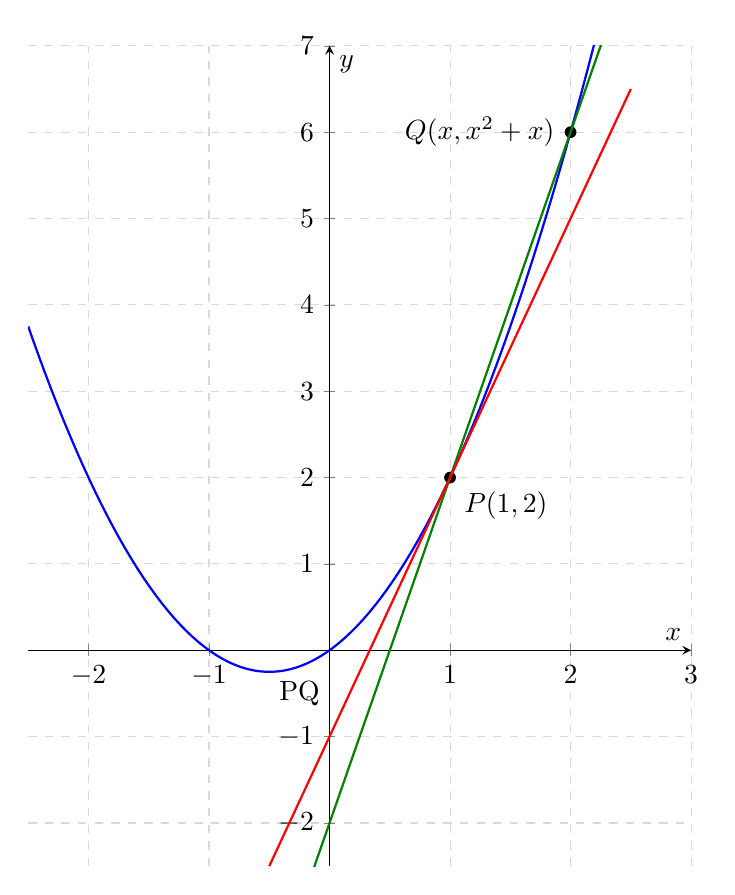
\begin{tikzpicture}
        \begin{axis}[
            axis lines=middle,
            xlabel=$x$,
            ylabel=$y$,
            xmin=-2.5, xmax=3,
            ymin=-2.5, ymax=7,
            legend pos=north west,
            grid=major,
            grid style={dashed, gray!30},
            width=10cm,
            height=12cm,
        ]
        
        % Đồ thị Parabol
        \addplot[domain=-2.5:2.5, samples=100, thick, blue, legend entries={$y=x^2+x$}] {x^2+x};
        
        % Điểm P và Q
        \node[circle, fill, inner sep=1.5pt, label={below right:$P(1,2)$}] at (axis cs:1,2) {};
        \node[circle, fill, inner sep=1.5pt, label={left:$Q(x, x^2+x)$}] at (axis cs:2,6) {};
        
        % Cát tuyến PQ
        \addplot[domain=-0.5:2.5, thick, green!50!black] {4*x-2};
        \node at (axis cs:0,-0.25) [anchor=north east] {PQ};

        % Tiếp tuyến t
        \addplot[domain=-0.5:2.5, thick, red, legend entries={$t$}] {3*x-1};
        
        \end{axis}
    \end{tikzpicture}
    \caption{Cát tuyến $PQ$ tiến dần về tiếp tuyến $t$ khi $Q \to P$.}
    \label{fig:tangent_of_parabola}
\end{figure}

    Ta có thể dự đoán một cách hợp lý rằng hệ số góc của tiếp tuyến tại $P$ chính là giới hạn của hệ số góc của cát tuyến $PQ$ khi $Q$ tiến về $P$. Tức là:
    \begin{equation*}
        m = \limit{x}{1} m_{PQ} = \limit{x}{1} (x+2) = 3
    \end{equation*}
    
    Với hệ số góc $m=3$ và đi qua điểm $P(1,2)$, phương trình đường tiếp tuyến là:
    \begin{equation*}
        y - 2 = 3(x-1) \quad \text{hay} \quad y = 3x - 1
    \end{equation*}
\end{solution}

Qua ví dụ trên, ta có thể rút ra một nhận định quan trọng: Tiếp tuyến tại điểm $P$ là vị trí giới hạn của cát tuyến $PQ$ khi điểm $Q$ tiến dần về $P$ dọc theo đường cong. Khái niệm ``giới hạn" này chính là chìa khóa để định nghĩa chính xác tiếp tuyến, vận tốc và nhiều đại lượng quan trọng khác trong giải tích.

% Nối tiếp vào file chapters/02 - chapter2.tex

\subsubsection{Bài toán vận tốc}

Khái niệm \textbf{vận tốc trung bình} rất quen thuộc: đó là tỉ số giữa quãng đường đi được và khoảng thời gian di chuyển. Tuy nhiên, khi ta lái xe, đồng hồ công - tơ - mét lại hiển thị một giá trị thay đổi liên tục, đó là \textbf{vận tốc tức thời} - vận tốc tại một thời điểm cụ thể. Vậy, vận tốc tức thời được định nghĩa chính xác như thế nào?

\begin{example}
    Một vật nhỏ được thả rơi tự do từ đỉnh một tòa tháp cao 200 mét. Bỏ qua sức cản không khí, quãng đường vật rơi được sau $t$ giây được cho bởi công thức:
    \[s(t) = \dfrac{1}{2}gt^2\]
    trong đó $g \approx 9,8 \text{ m/s}^2$ là gia tốc trọng trường. Hãy xác định vận tốc của vật sau 3 giây.
\end{example}

\begin{solution}
    Ta có công thức quãng đường là $s(t) = 4,9t^2$. Để tìm vận tốc tức thời tại thời điểm $t=3$ giây, ta có thể xấp xỉ nó bằng cách tính vận tốc trung bình trên một khoảng thời gian rất ngắn bắt đầu từ $t=3$. Ví dụ, trên khoảng thời gian từ $t=3$ đến $t=3,1$ giây:
    \begin{equation*}
        \text{Vận tốc trung bình} = \dfrac{\text{Quãng đường đi được}}{\text{Thời gian di chuyển}} = \dfrac{s(3,1) - s(3)}{3,1 - 3}
    \end{equation*}
    \begin{equation*}
        = \dfrac{4,9(3,1)^2 - 4,9(3)^2}{0,1} = \dfrac{47,089 - 44,1}{0,1} = 29,89 \text{ m/s}
    \end{equation*}
    
    Bảng dưới đây cho thấy các giá trị vận tốc trung bình được tính trên các khoảng thời gian ngày càng nhỏ hơn:
    
    \begin{center}
        \begin{tabular}{|l|c|}
            \hline
            \textbf{Khoảng thời gian (s)} & \textbf{Vận tốc trung bình (m/s)} \\
            \hline
            $3 \le t \le 4$ & $34,3$ \\
            $3 \le t \le 3,1$ & $29,89$ \\
            $3 \le t \le 3,01$ & $29,449$ \\
            $3 \le t \le 3,001$ & $29,4049$ \\
            $3 \le t \le 3,0001$ & $29,40049$ \\
            \hline
        \end{tabular}
    \end{center}
    
    Dữ liệu từ bảng cho thấy khi khoảng thời gian co lại dần về 0, vận tốc trung bình dường như đang tiến rất gần đến giá trị $29,4 \text{ m/s}$. Do đó, ta có thể dự đoán rằng vận tốc tức thời của vật tại thời điểm $t=3$ giây chính là $29,4 \text{ m/s}$.
    
    Từ đó, ta đi đến một kết luận tương tự như bài toán tiếp tuyến: Vận tốc tức thời tại thời điểm $t$ chính là ``giới hạn" của vận tốc trung bình trên khoảng thời gian từ $t$ đến $t'$ khi $t'$ ``tiến về" $t$.
\end{solution}

\subsubsection{Tỉ lệ thay đổi}

Cả hai bài toán tìm hệ số góc của tiếp tuyến và tìm vận tốc tức thời đều dẫn chúng ta đến một khái niệm chung: tìm ``giới hạn" của một đại lượng có dạng:
\begin{equation*}
    \dfrac{f(x) - f(a)}{x - a}
\end{equation*}
khi $x$ ``tiến về" $a$.

Giá trị giới hạn này biểu diễn tỉ lệ thay đổi tức thời của đại lượng $f(x)$ so với sự thay đổi của đại lượng $x$ tại giá trị $x=a$. Đây là một khái niệm nền tảng, là công cụ chủ chốt của phép tính vi tích phân để khảo sát các hiện tượng biến đổi trong thế giới thực. Đại lượng này được gọi là đạo hàm, và chúng ta sẽ nghiên cứu sâu hơn về nó trong chương tiếp theo.

Tuy nhiên, để có thể xây dựng một cách chặt chẽ khái niệm đạo hàm, trước hết chúng ta cần phải định nghĩa chính xác khái niệm ``giới hạn". Đây chính là nội dung chúng ta sẽ tìm hiểu ngay sau đây.

% Nối tiếp vào file chapters/02 - chapter2.tex

\subsection{Giới hạn của hàm số}
\label{subsec:dinh-nghia-gioi-han}

Ý niệm về giới hạn và sự hội tụ đã manh nha từ thời cổ đại, chẳng hạn như Archimedes đã sử dụng ý tưởng rằng chu vi của một đường tròn là ``giới hạn'' của chu vi của một đa giác đều nội tiếp khi số cạnh của nó tăng lên vô hạn.

Một cách trực quan, ta nói ``giới hạn của hàm số $f(x)$ khi $x$ tiến về $a$ là $L$'', nếu ta có thể làm cho giá trị của $f(x)$ gần với $L$ một cách tùy ý bằng cách chọn $x$ đủ gần $a$ (nhưng không bằng $a$). Ta ký hiệu điều này là:
\begin{equation*}
    \limit{x}{a} f(x) = L
\end{equation*}

Trong nhiều trường hợp, ta có thể hiểu một cách đơn giản hơn: nếu $x$ càng gần $a$ thì $f(x)$ càng gần $L$.

\begin{example}
    Cho $f(x) = c$ là một hàm hằng. Khi $x$ tiến đến một giá trị $a$ bất kỳ, giá trị của $f(x)$ luôn luôn bằng $c$. Do đó, một cách tự nhiên ta có:
    \begin{equation*}
        \limit{x}{a} c = c
    \end{equation*}
\end{example}

\begin{example}
    Cho $f(x) = x$. Rõ ràng, khi $x$ tiến gần đến $a$, giá trị của $f(x)$ (chính là $x$) cũng tiến gần đến $a$. Vậy:
    \begin{equation*}
        \limit{x}{a} x = a
    \end{equation*}
\end{example}

Một điểm cực kỳ quan trọng trong định nghĩa giới hạn là ta chỉ quan tâm đến giá trị của $f(x)$ khi $x$ \textit{lân cận} $a$, chứ không phải giá trị của $f(x)$ \textit{tại} $x=a$. Điều này cho phép chúng ta xét giới hạn tại những điểm mà hàm số không xác định.

\begin{example}
    Xét giới hạn $\limit{x}{1} \dfrac{x^2 - 1}{x - 1}$.
    
    Hàm số $f(x) = \dfrac{x^2 - 1}{x - 1}$ không xác định tại $x=1$. Tuy nhiên, khi $x$ gần 1 nhưng $x \neq 1$, ta có thể rút gọn biểu thức:
    \begin{equation*}
        \dfrac{x^2 - 1}{x - 1} = \dfrac{(x-1)(x+1)}{x-1} = x+1
    \end{equation*}
    Do đó, giới hạn của hàm số ban đầu sẽ bằng giới hạn của hàm số $g(x) = x+1$ khi $x \to 1$:
    \begin{equation*}
        \limit{x}{1} \dfrac{x^2 - 1}{x - 1} = \limit{x}{1} (x+1) = 1+1 = 2
    \end{equation*}
\end{example}
    
\begin{figure}[H]
    \centering
    \begin{tikzpicture}
        \begin{axis}[
            axis lines=middle,
            xlabel=$x$, ylabel=$y$,
            xmin=-1.5, xmax=3.5,
            ymin=-0.5, ymax=4.5,
            xtick={1}, ytick={2},
            grid=major,
            grid style={dashed, gray!30},
            width=8cm, height=6cm,
        ]
        
        \addplot[domain=-1.2:3, samples=100, thick, blue, name path=f] {x+1};
        \node[label={above right:$y=\frac{x^2-1}{x-1}$}] at (axis cs:1.8, 2) {};
        
        % Điểm không xác định
        \node[circle, draw, fill=white, inner sep=1.5pt] at (axis cs:1,2) {};
        
        % Dóng xuống trục
        \draw[dashed, violet] (axis cs:1,0) -- (axis cs:1,2) -- (axis cs:0,2);
        
        % Mũi tên chỉ sự tiến đến
        \draw[->, red, thick] (axis cs:0.6, -0.4) -- (axis cs:0.9, -0.4);
        \draw[->, red, thick] (axis cs:1.4, -0.4) -- (axis cs:1.1, -0.4);
        \draw[->, red, thick] (axis cs:-0.25, 1.4) -- (axis cs:-0.25, 1.8);
        \draw[->, red, thick] (axis cs:-0.25, 2.6) -- (axis cs:-0.25, 2.2);

        \end{axis}
    \end{tikzpicture}
    \caption{Đồ thị hàm số $y=\frac{x^2-1}{x-1}$ có một ``lỗ hổng'' tại $x=1$.\footnotemark}
    \label{fig:gioi-han-lo-hong}
\end{figure}
\footnotetext{dấu tròn rỗng biểu diễn điểm đó không nằm trên (không thuộc) đồ thị}

Ví dụ trên một lần nữa nhấn mạnh rằng: \textbf{giới hạn của $f(x)$ khi $x \to a$ không phụ thuộc vào giá trị của $f(a)$}. Hàm $f$ thậm chí không cần xác định tại $a$. Giới hạn chỉ phụ thuộc vào hành vi của hàm số ở \textit{lân cận} của $a$. Hình \ref{fig:gioi-han-khong-phu-thuoc-f(a)} minh họa rõ điều này.

\begin{figure}[H]
    \centering
    \begin{tikzpicture}[scale=1.2]
        % (a) f(a) = L
        \begin{scope}[xshift=-4cm]
            \draw[->] (-1.5,0) -- (1.5,0) node[right] {$x$};
            \draw[->] (0,-1) -- (0,2) node[above] {$y$};
            \draw[thick, blue] plot[smooth, tension=0.8] coordinates {(-1.2, -0.5) (-0.5, 1.2) (0.5, 0.8) (1.2, 1.5)};
            \draw[dashed] (0.5,0) node[below] {$a$} -- (0.5,0.8) -- (0,0.8) node[left] {$L$};
            \node[circle, fill, inner sep=1.2pt] at (0.5,0.8) {};
            \node at (0, -1.5) {(a)};
        \end{scope}

        % (b) f(a) != L
        \begin{scope}
            \draw[->] (-1.5,0) -- (1.5,0) node[right] {$x$};
            \draw[->] (0,-1) -- (0,2) node[above] {$y$};
            \draw[thick, blue] plot[smooth, tension=0.8] coordinates {(-1.2, -0.5) (-0.5, 1.2) (0.5, 0.8) (1.2, 1.5)};
            \draw[dashed] (0.5,0) node[below] {$a$} -- (0.5,0.8) -- (0,0.8) node[left] {$L$};
            \node[circle, draw, fill=white, inner sep=1.2pt] at (0.5,0.8) {};
            \node[circle, fill, inner sep=1.2pt, blue] at (0.5, 0.2) {};
            \node at (0, -1.5) {(b)};
        \end{scope}

        % (c) f(a) không xác định
        \begin{scope}[xshift=4cm]
            \draw[->] (-1.5,0) -- (1.5,0) node[right] {$x$};
            \draw[->] (0,-1) -- (0,2) node[above] {$y$};
            \draw[thick, blue] plot[smooth, tension=0.8] coordinates {(-1.2, -0.5) (-0.5, 1.2) (0.5, 0.8) (1.2, 1.5)};
            \draw[dashed] (0.5,0) node[below] {$a$} -- (0.5,0.8) -- (0,0.8) node[left] {$L$};
            \node[circle, draw, fill=white, inner sep=1.2pt] at (0.5,0.8) {};
            \node at (0, -1.5) {(c)};
        \end{scope}
    \end{tikzpicture}
    \caption{Trong cả ba trường hợp, $\limit{x}{a} f(x) = L$.}
    \label{fig:gioi-han-khong-phu-thuoc-f(a)}
\end{figure}

\subsubsection{Định nghĩa chính xác của giới hạn}

Để có thể xây dựng nền tảng vững chắc cho giải tích, khái niệm giới hạn cần được định nghĩa một cách chặt chẽ bằng ngôn ngữ toán học. Định nghĩa này, thường được gọi là ``định nghĩa $\epsilon-\delta$'', tuy có vẻ trừu tượng lúc ban đầu, nhưng nó chính là công cụ để lượng hóa ý tưởng trực quan ``càng gần'' mà chúng ta đã thảo luận, cho phép chúng ta chứng minh các tính chất phức tạp một cách rigua.

Trước hết, ta cần một khái niệm về điểm mà tại đó việc xét giới hạn là có ý nghĩa.

\begin{definition}[Điểm tụ]
    Một điểm $a$ được gọi là một \textbf{điểm tụ} (hay \textbf{điểm giới hạn}) của tập hợp $D \subset \R$ nếu mọi khoảng mở chứa $a$ đều chứa ít nhất một điểm của $D$ khác $a$.
\end{definition}

Nói một cách khác, $a$ là điểm tụ của $D$ nếu luôn có những phần tử của $D$ (khác $a$) nằm gần $a$ một cách tùy ý. Lưu ý rằng một điểm tụ của $D$ không nhất thiết phải thuộc $D$.

\begin{example}
    Cùng xem xét một số trường hợp sau:
    \begin{itemize}
        \item Điểm 0 là một điểm tụ của tập $(0, 1)$ và cũng là điểm tụ của tập $\R \setminus \{0\}$.
        \item Tập hợp $\{1, 2, 3\}$ không có điểm tụ nào.
        \item Mọi điểm trong khoảng $[0,1]$ đều là điểm tụ của khoảng $(0,1)$.
    \end{itemize}
\end{example}

\noindent Bây giờ, chúng ta có thể phát biểu định nghĩa chính xác của giới hạn.

\begin{definition}[Giới hạn của hàm số]
    \label{def:epsilon-delta}
    Cho hàm số $f$ xác định trên tập $D$ và $a$ là một điểm tụ của $D$. Ta nói \textbf{giới hạn của $f(x)$ khi $x$ tiến đến $a$ là $L$}, và viết là
    \begin{equation*}
        \limit{x}{a} f(x) = L
    \end{equation*}
    nếu với mọi số thực $\epsilon > 0$, tồn tại một số thực $\delta > 0$ sao cho với mọi $x \in D$, nếu $0 < \abs{x-a} < \delta$ thì $\abs{f(x) - L} < \epsilon$.
    
    Dưới dạng ký hiệu logic:
    \begin{equation*}
        \forall \epsilon > 0, \exists \delta > 0, \forall x \in D, (0 < \abs{x-a} < \delta \implies \abs{f(x) - L} < \epsilon)
    \end{equation*}
\end{definition}

\begin{figure}[H]
    \centering
    \begin{tikzpicture}
        % Trục x
        \draw[->] (-3,0) -- (3,0) node[right] {};
        \node at (0,0) [below=3pt] {$a$};
        \draw (0, -0.1) -- (0, 0.1);
        \draw[red] (-1.5, 0.1) -- (-1.5, -0.1) node[below] {$a-\delta$};
        \draw[red] (1.5, 0.1) -- (1.5, -0.1) node[below] {$a+\delta$};
        \draw[red, dashed] (-1.5, 0) -- (1.5, 0);
        \node at (-0.5, 0.3) [above] {$x$};
        \filldraw[black] (-0.5,0) circle (1.5pt);

        % Trục y
        \draw[->] (5,0) -- (11,0) node[right] {};
        \node at (8,0) [below=3pt] {$L$};
        \draw (8, -0.1) -- (8, 0.1);
        \draw[red] (6, 0.1) -- (6, -0.1) node[below] {$L-\epsilon$};
        \draw[red] (10, 0.1) -- (10, -0.1) node[below] {$L+\epsilon$};
        \draw[red, dashed] (6, 0) -- (10, 0);
        \node at (8.8, 0.3) [above] {$f(x)$};
        \filldraw[black] (8.8,0) circle (1.5pt);
        
        % Ánh xạ f
        \draw[->, thick, blue!60] (-0.5, 0) .. controls (4, 2.5) and (7, 2.5) .. (8.8, 0) node[midway, above] {$f$};
    \end{tikzpicture}
    \caption{Minh họa định nghĩa $\epsilon-\delta$ của giới hạn.}
    \label{fig:epsilon-delta}
\end{figure}

Định nghĩa này nói rằng: bạn có thể làm cho sai số $\abs{f(x)-L}$ nhỏ hơn bất kỳ một ngưỡng dương $\epsilon$ nào bạn muốn, miễn là bạn chọn $x$ đủ gần $a$ (tức là trong khoảng $(a-\delta, a+\delta)$), nhưng không phải là $a$.

\begin{example}
    Sử dụng định nghĩa $\epsilon-\delta$ để chứng minh rằng $\limit{x}{3} (3x - 2) = 7$.
\end{example}
\textbf{Bước 1 Đoán $\delta$:} Cho trước một $\epsilon > 0$ bất kỳ. Ta cần tìm một số $\delta > 0$ sao cho:
\begin{center}
    nếu $0 < \abs{x-3} < \delta$ thì $\abs{(3x-2) - 7} < \epsilon$.
\end{center}
Ta biến đổi vế phải của bất đẳng thức:
\begin{equation*}
    \abs{(3x-2) - 7} = \abs{3x - 9} = 3\abs{x-3}
\end{equation*}
Như vậy, ta muốn $3\abs{x-3} < \epsilon$, điều này tương đương với $\abs{x-3} < \dfrac{\epsilon}{3}$.
Điều này gợi ý cho ta nên chọn $\delta = \dfrac{\epsilon}{3}$.

\textbf{Bước 2 Chứng minh:} Cho trước $\epsilon > 0$. Ta chọn $\delta = \dfrac{\epsilon}{3}$.
Khi đó, với mọi $x$ thỏa mãn $0 < \abs{x-3} < \delta$, ta có:
\begin{equation*}
    \abs{(3x-2) - 7} = 3\abs{x-3} < 3\delta = 3\left(\dfrac{\epsilon}{3}\right) = \epsilon
\end{equation*}
Theo định nghĩa \ref{def:epsilon-delta}, ta đã chứng minh được $\limit{x}{3} (3x - 2) = 7$.

\begin{example}
    Chứng minh rằng $\limit{x}{3} x^2 = 9$.
\end{example}

\textbf{1. Phân tích (tìm $\delta$):} Cho trước $\epsilon > 0$. Ta cần tìm $\delta > 0$ sao cho nếu $0 < \abs{x-3} < \delta$ thì $\abs{x^2 - 9} < \epsilon$.
Ta có $\abs{x^2 - 9} = \abs{x-3}\abs{x+3}$.

Ở đây, thừa số $\abs{x+3}$ không phải là hằng số. Tuy nhiên, vì ta chỉ quan tâm đến các giá trị $x$ gần 3, ta có thể giới hạn $x$ trong một khoảng nào đó quanh 3, ví dụ, ta yêu cầu $\delta \le 1$.
Nếu $\abs{x-3} < 1$, thì $-1 < x-3 < 1$, hay $2 < x < 4$.
Điều này suy ra $5 < x+3 < 7$, do đó $\abs{x+3} < 7$.

Bây giờ, ta có: $\abs{x^2 - 9} = \abs{x-3}\abs{x+3} < 7\abs{x-3}$.
Để $7\abs{x-3} < \epsilon$, ta cần $\abs{x-3} < \dfrac{\epsilon}{7}$.

Vậy, ta cần cả hai điều kiện: $\abs{x-3} < 1$ và $\abs{x-3} < \dfrac{\epsilon}{7}$. Ta có thể chọn $\delta$ là giá trị nhỏ hơn trong hai số $1$ và $\dfrac{\epsilon}{7}$, tức là $\delta = \min\left\{1, \dfrac{\epsilon}{7}\right\}$.

\textbf{2. Chứng minh:} Cho trước $\epsilon > 0$. Chọn $\delta = \min\left\{1, \dfrac{\epsilon}{7}\right\}$.
Nếu $0 < \abs{x-3} < \delta$, thì ta có $\abs{x-3} < 1$ và $\abs{x-3} < \dfrac{\epsilon}{7}$.
Vì $\abs{x-3} < 1$, ta suy ra $\abs{x+3} < 7$ (như đã phân tích ở trên).
Do đó:
\begin{equation*}
    \abs{x^2 - 9} = \abs{x-3}\abs{x+3} < \left(\dfrac{\epsilon}{7}\right) \cdot 7 = \epsilon
\end{equation*}
Vậy, theo định nghĩa, $\limit{x}{3} x^2 = 9$.

Việc yêu cầu $a$ phải là một điểm tụ của miền xác định đảm bảo một tính chất quan trọng: giới hạn nếu tồn tại thì phải là duy nhất.

\begin{proposition}[Tính duy nhất của giới hạn]
    Nếu $\limit{x}{a} f(x) = L_1$ và $\limit{x}{a} f(x) = L_2$ thì $L_1 = L_2$.
\end{proposition}
\begin{proof}
    Giả sử $L_1 \neq L_2$. Đặt $\epsilon = \dfrac{\abs{L_1 - L_2}}{2} > 0$.
    \begin{itemize}
        \item Vì $\limit{x}{a} f(x) = L_1$, tồn tại $\delta_1 > 0$ sao cho nếu $0 < \abs{x-a} < \delta_1$ thì $\abs{f(x) - L_1} < \epsilon$.
        \item Vì $\limit{x}{a} f(x) = L_2$, tồn tại $\delta_2 > 0$ sao cho nếu $0 < \abs{x-a} < \delta_2$ thì $\abs{f(x) - L_2} < \epsilon$.
    \end{itemize}
    Chọn $\delta = \min\{\delta_1, \delta_2\}$. Vì $a$ là điểm tụ, tồn tại một $x_0 \in D$ sao cho $0 < \abs{x_0 - a} < \delta$.
    Với $x_0$ này, ta có cả $\abs{f(x_0) - L_1} < \epsilon$ và $\abs{f(x_0) - L_2} < \epsilon$.
    Sử dụng bất đẳng thức tam giác, ta có:
    \begin{equation*}
        \abs{L_1 - L_2} = \abs{L_1 - f(x_0) + f(x_0) - L_2} \le \abs{f(x_0) - L_1} + \abs{f(x_0) - L_2} < \epsilon + \epsilon = 2\epsilon
    \end{equation*}
    Thay $\epsilon = \dfrac{\abs{L_1 - L_2}}{2}$ vào, ta được $\abs{L_1 - L_2} < 2 \cdot \dfrac{\abs{L_1 - L_2}}{2} = \abs{L_1 - L_2}$.
    Đây là một điều mâu thuẫn. Do đó, giả sử ban đầu là sai, và ta phải có $L_1 = L_2$.
\end{proof}

Có thể thấy, việc chứng minh giới hạn trực tiếp từ định nghĩa $\epsilon-\delta$ khá phức tạp và đòi hỏi nhiều kỹ thuật. May mắn là, từ định nghĩa này, chúng ta có thể xây dựng nên các định lý và quy tắc tính toán, giúp cho việc tìm giới hạn trở nên đơn giản hơn rất nhiều, như chúng ta sẽ thấy ở mục tiếp theo.

% Nối tiếp vào file chapters/02 - chapter2.tex

\subsection{Một số tính chất căn bản của giới hạn}
\label{subsec:tinh-chat-gioi-han}

Việc sử dụng định nghĩa $\epsilon-\delta$ để chứng minh mọi giới hạn là không thực tế. Thay vào đó, chúng ta sẽ xây dựng một bộ các quy tắc và định lý cho phép tính toán giới hạn một cách hiệu quả hơn. Các tính chất này hoàn toàn tương tự với các tính chất của giới hạn dãy số đã được trình bày trong Định lý~\ref{thm:limit-preserve-operations}.

\begin{theorem}[Các quy tắc tính giới hạn]
    \label{thm:limit-laws}
    Giả sử rằng $\limit{x}{a} f(x)$ và $\limit{x}{a} g(x)$ đều tồn tại. Khi đó:
    \begin{enumerate}[label=(\alph*)]
        \item $\limit{x}{a} [f(x) + g(x)] = \limit{x}{a} f(x) + \limit{x}{a} g(x)$
        \item $\limit{x}{a} [f(x) - g(x)] = \limit{x}{a} f(x) - \limit{x}{a} g(x)$
        \item $\limit{x}{a} [f(x) \cdot g(x)] = \left(\limit{x}{a} f(x)\right) \cdot \left(\limit{x}{a} g(x)\right)$
        \item $\limit{x}{a} \dfrac{f(x)}{g(x)} = \dfrac{\limit{x}{a} f(x)}{\limit{x}{a} g(x)}$, nếu $\limit{x}{a} g(x) \neq 0$.
    \end{enumerate}
\end{theorem}
\begin{proof} Như đã nói bên trên, vì tính chất gần tương tự, nên ta có thể chứng minh mệnh đề tương ứng cho giới hạn ở Định lý~\ref{thm:limit-preserve-operations}

    Đặt $L = \limit{x}{a} f(x)$ và $M = \limit{x}{a} g(x)$. Cho trước $\epsilon > 0$.
    Ta cần chỉ ra rằng:
    \[\abs{(f(x)+g(x)) - (L+M)}\]
    có thể nhỏ tùy ý. Sử dụng bất đẳng thức tam giác:
    \begin{equation*}
        \abs{(f(x)+g(x)) - (L+M)} = \abs{(f(x)-L) + (g(x)-M)} \le \abs{f(x)-L} + \abs{g(x)-M}
    \end{equation*}
    Vì $f(x) \to L$, ta có thể làm cho $\abs{f(x)-L} < \dfrac{\epsilon}{2}$. Tương tự, ta có thể làm cho $\abs{g(x)-M} < \dfrac{\epsilon}{2}$.
    Do đó, ta có thể làm cho tổng của chúng nhỏ hơn $\dfrac{\epsilon}{2} + \dfrac{\epsilon}{2} = \epsilon$. Lập luận chi tiết hoàn toàn tương tự như chứng minh cho giới hạn dãy số.
\end{proof}

Các quy tắc trên cho phép chúng ta tính giới hạn của các hàm phức tạp bằng cách chia chúng thành các phần đơn giản hơn.

\begin{example}
    Tính $\limit{x}{1} (2x^2 + 3x - 1)$.
    
    Áp dụng các quy tắc tính giới hạn, ta có:
    \begin{align*}
        \limit{x}{1} (2x^2 + 3x - 1) &= \limit{x}{1} (2x^2) + \limit{x}{1} (3x) - \limit{x}{1} (1) \\
        &= 2 \left(\limit{x}{1} x\right)^2 + 3 \left(\limit{x}{1} x\right) - 1 \\
        &= 2(1)^2 + 3(1) - 1 = 4.
    \end{align*}
\end{example}

Ví dụ trên cho thấy một nguyên tắc quan trọng: đối với hàm đa thức $P(x)$, giới hạn của nó khi $x \to a$ có thể được tìm thấy bằng cách thay thế trực tiếp: $\limit{x}{a} P(x) = P(a)$. Tương tự, đối với hàm phân thức hữu tỉ $f(x) = P(x)/Q(x)$, ta có:
\begin{equation*}
    \limit{x}{a} \dfrac{P(x)}{Q(x)} = \dfrac{P(a)}{Q(a)}, \quad \text{miễn là } Q(a) \neq 0.
\end{equation*}

\begin{example}
    Tìm giới hạn $\limit{x}{2} \dfrac{x^2 - 4}{x - 2}$.
    
    Ở đây, ta không thể thay $x=2$ vào ngay vì mẫu số sẽ bằng 0. Tuy nhiên, vì giới hạn không phụ thuộc vào giá trị của hàm tại chính điểm đó, ta có thể rút gọn biểu thức khi $x \neq 2$:
    \begin{equation*}
        \dfrac{x^2 - 4}{x - 2} = \dfrac{(x-2)(x+2)}{x-2} = x+2
    \end{equation*}
    Do đó,
    \begin{equation*}
        \limit{x}{2} \dfrac{x^2 - 4}{x - 2} = \limit{x}{2} (x+2) = 2+2 = 4.
    \end{equation*}
\end{example}

Bên cạnh các quy tắc tính toán, chúng ta còn có các định lý so sánh, tương tự như đối với giới hạn dãy số.

% TODO link voi cai gioi han day so.

\begin{theorem}[Tính chất so sánh]
    \label{thm:comparison-property}
    Nếu $f(x) \le g(x)$ khi $x$ ở lân cận $a$ (có thể ngoại trừ tại $a$) và các giới hạn của $f$ và $g$ tại $a$ đều tồn tại, thì:
    \begin{equation*}
        \limit{x}{a} f(x) \le \limit{x}{a} g(x)
    \end{equation*}
\end{theorem}

Từ định lý này, ta có một hệ quả cực kỳ hữu ích, thường được gọi là Định lý Kẹp.

\begin{corollary}[Định lý Kẹp]
    \label{cor:squeeze-theorem}
    Nếu $f(x) \le g(x) \le h(x)$ khi $x$ ở lân cận $a$ (có thể ngoại trừ tại $a$), và 
    \(\limit{x}{a} f(x) = \limit{x}{a} h(x) = L\)
    thì 
    \[\limit{x}{a} g(x) = L\]
\end{corollary}

\begin{example}
    Tìm giới hạn $\limit{x}{0} x^2 \cos\left(\dfrac{\pi}{x}\right)$.
    
    Ta biết rằng hàm cosin luôn bị chặn trong đoạn $[-1, 1]$. Do đó, với mọi $x \neq 0$:
    
    \begin{equation*}
        -1 \le \cos\left(\dfrac{\pi}{x}\right) \le 1
    \end{equation*}
    
    Nhân tất cả các vế với $x^2$ (lưu ý $x^2 \ge 0$), ta được:
    \begin{equation*}
        -x^2 \le x^2 \cos\left(\dfrac{\pi}{x}\right) \le x^2
    \end{equation*}
    
    Ta có $\limit{x}{0} (-x^2) = 0$ và $\limit{x}{0} x^2 = 0$.
    
    Theo Định lý Kẹp, ta kết luận:
    \begin{equation*}
        \limit{x}{0} x^2 \cos\left(\dfrac{\pi}{x}\right) = 0
    \end{equation*}
\end{example}

\subsubsection{* Giới hạn của hàm số thông qua giới hạn của dãy số}
\label{subsec:gioi-han-qua-day-so}

Ngoài định nghĩa $\epsilon-\delta$, có một cách tiếp cận khác để định nghĩa giới hạn của hàm số thông qua giới hạn của dãy số. Cách tiếp cận này có thể quen thuộc hơn với người đọc từ Mục \ref{subsec:day_so_thuc} và cũng là phương pháp được sử dụng trong sách giáo khoa phổ thông [SGKTH]. Mối liên hệ này được phát biểu qua mệnh đề sau.

\begin{proposition}
    \label{prop:sequential-characterization-limit}
    Cho $a$ là một điểm tụ của miền xác định của hàm số $f$. Hai mệnh đề sau là tương đương:
    \begin{enumerate}[label=(\alph*)]
        \item $\limit{x}{a} f(x) = L$.
        \item Với mọi dãy số $(x_n)_{n \ge 1}$ trong miền xác định của $f$ (với $x_n \neq a$) hội tụ về $a$, thì dãy các giá trị tương ứng $(f(x_n))_{n \ge 1}$ hội tụ về $L$. Nói cách khác:
        \begin{equation*}
            \text{Nếu } \limit{n}{\infty} x_n = a \text{ thì } \limit{n}{\infty} f(x_n) = L.
        \end{equation*}
    \end{enumerate}
\end{proposition}
\begin{proof}
    Chứng minh của mệnh đề này không quá phức tạp và có thể được tìm thấy trong các tài liệu giải tích chuyên sâu hơn như [Kha96].
\end{proof}

Mệnh đề này rất hữu ích. Nó cho phép chúng ta suy ra các tính chất của giới hạn hàm số (như các quy tắc tính giới hạn ở mục trước) một cách trực tiếp từ các tính chất tương ứng của giới hạn dãy số.

Một ứng dụng quan trọng khác là dùng mệnh đề này để chứng minh một hàm số \textit{không} có giới hạn tại một điểm.

\begin{corollary}
    \label{cor:khong-ton-tai-gioi-han}
    Hàm số $f$ không có giới hạn tại $a$ nếu xảy ra một trong hai trường hợp sau:
    \begin{enumerate}[label=(\alph*)]
        \item Tồn tại một dãy $(x_n)_{n \ge 1}$ sao cho $\limit{n}{\infty} x_n = a$ nhưng dãy $(f(x_n))_{n \ge 1}$ phân kỳ.
        \item Tồn tại hai dãy $(x_n)_{n \ge 1}$ và $(y_n)_{n \ge 1}$ sao cho
        \begin{equation*}
            \limit{n}{\infty} x_n = \limit{n}{\infty} y_n = a
        \end{equation*}
        nhưng
        \begin{equation*}
            \limit{n}{\infty} f(x_n) \neq \limit{n}{\infty} f(y_n).
        \end{equation*}
    \end{enumerate}
\end{corollary}

\begin{example}
    Chứng tỏ rằng $\limit{x}{0} \cos\left(\dfrac{1}{x}\right)$ không tồn tại.
\end{example}
\begin{solution}
    Để chứng minh giới hạn này không tồn tại, ta sẽ chỉ ra hai dãy số cùng tiến về 0, nhưng giá trị của hàm tại hai dãy đó lại tiến về hai giới hạn khác nhau, theo Hệ quả \ref{cor:khong-ton-tai-gioi-han}(b).
    
    \begin{itemize}
        \item Chọn dãy thứ nhất: $x_n = \dfrac{1}{2n\pi}$, với $n \in \N, n \ge 1$.
        Khi $n \to \infty$, rõ ràng $x_n \to 0$.
        Giá trị của hàm tại dãy này là:
        \begin{equation*}
            f(x_n) = \cos\left(\dfrac{1}{x_n}\right) = \cos(2n\pi) = 1, \quad \forall n \ge 1.
        \end{equation*}
        Do đó, $\limit{n}{\infty} f(x_n) = 1$.
        
        \item Chọn dãy thứ hai: $y_n = \dfrac{1}{(2n+1)\pi}$, với $n \in \N, n \ge 0$.
        Khi $n \to \infty$, $y_n \to 0$.
        Giá trị của hàm tại dãy này là:
        \begin{equation*}
            f(y_n) = \cos\left(\dfrac{1}{y_n}\right) = \cos((2n+1)\pi) = -1, \quad \forall n \ge 0.
        \end{equation*}
        Do đó, $\limit{n}{\infty} f(y_n) = -1$.
    \end{itemize}
    
    Vì ta đã tìm thấy hai dãy $(x_n)$ và $(y_n)$ cùng tiến về 0 nhưng dãy các giá trị hàm tương ứng lại tiến về hai giới hạn khác nhau ($1 \neq -1$), ta kết luận rằng giới hạn $\limit{x}{0} \cos\left(\dfrac{1}{x}\right)$ không tồn tại.
\end{solution}

% Nối tiếp vào file chapters/02 - chapter2.tex

\subsection{Các giới hạn mở rộng}
\label{subsec:gioi-han-mo-rong}

\subsubsection{Giới hạn một phía}

Trong nhiều trường hợp, hành vi của một hàm số khi tiến đến một điểm có thể khác nhau tùy thuộc vào việc ta tiếp cận từ bên trái hay bên phải. Chẳng hạn, xét hàm số được định nghĩa bởi:
\begin{equation*}
    f(x) = \begin{cases}
        -1, & \text{nếu } x < 0 \\
        1,  & \text{nếu } x > 0
    \end{cases}
\end{equation*}
Khi $x$ tiến về 0 từ phía các số âm (bên trái), $f(x)$ luôn bằng $-1$. Nhưng khi $x$ tiến về 0 từ phía các số dương (bên phải), $f(x)$ luôn bằng $1$. Điều này thúc đẩy chúng ta định nghĩa khái niệm giới hạn một phía.

\begin{definition} (Giới hạn một phía)
    \begin{itemize}
        \item Ta viết $\limit{x}{a^{-}} f(x) = L$ và nói \textbf{giới hạn bên trái} của $f(x)$ khi $x$ tiến đến $a$ là $L$, nếu ta có thể làm cho $f(x)$ gần $L$ tùy ý bằng cách chọn $x$ đủ gần $a$ và $x < a$. Bằng ký hiệu ta viết:
        \[\forall \epsilon > 0, \exists \delta > 0, \forall x \in D, -\delta < x - a < 0 \Rightarrow \abs{f(x) - L} < \epsilon\]
        
        \item Ta viết $\limit{x}{a^{+}} f(x) = L$ và nói \textbf{giới hạn bên phải} của $f(x)$ khi $x$ tiến đến $a$ là $L$, nếu ta có thể làm cho $f(x)$ gần $L$ tùy ý bằng cách chọn $x$ đủ gần $a$ và $x > a$. Bằng ký hiệu ta viết:
        \[\forall \epsilon > 0, \exists \delta > 0, \forall x \in D, 0 < x - a < \delta \Rightarrow \abs{f(x) - L} < \epsilon\]
    \end{itemize}
\end{definition}

Ký hiệu $x \to a^{-}$ có nghĩa là ta chỉ xét các giá trị $x$ nhỏ hơn $a$, và tương tự $x \to a^{+}$ có nghĩa là ta chỉ xét các giá trị $x$ lớn hơn $a$.

\begin{example}
    Xét hàm số $f(x) = \begin{cases} x+1, & \text{nếu } x < 1 \\ x^2, & \text{nếu } x > 1 \end{cases}$.
    
    Ta có:
    \begin{itemize}
        \item Giới hạn bên trái tại $x=1$: $\limit{x}{1^{-}} f(x) = \limit{x}{1^{-}} (x+1) = 2$.
        \item Giới hạn bên phải tại $x=1$: $\limit{x}{1^{+}} f(x) = \limit{x}{1^{+}} x^2 = 1$.
    \end{itemize}
\end{example}

Mối liên hệ giữa giới hạn hai phía (mà chúng ta đã định nghĩa trước đó) và giới hạn một phía được thể hiện qua mệnh đề sau.

\begin{proposition}
    \label{prop:limit-one-sided}
    Giới hạn $\limit{x}{a} f(x) = L$ tồn tại khi và chỉ khi cả hai giới hạn một phía đều tồn tại và bằng nhau, tức là:
    \begin{equation*}
        \limit{x}{a^{-}} f(x) = \limit{x}{a^{+}} f(x) = L
    \end{equation*}
\end{proposition}
\begin{proof}
    Mệnh đề này là một hệ quả trực tiếp từ định nghĩa $\epsilon-\delta$.
    \begin{itemize}
        \item $(\Rightarrow)$ Nếu $\limit{x}{a} f(x) = L$, thì với mọi $\epsilon > 0$, tồn tại $\delta > 0$ sao cho nếu $0 < \abs{x-a} < \delta$ thì $\abs{f(x)-L} < \epsilon$. Điều này hiển nhiên đúng cho cả trường hợp $a-\delta < x < a$ (giới hạn trái) và $a < x < a+\delta$ (giới hạn phải).
        \item $(\Leftarrow)$ Ngược lại, giả sử cả hai giới hạn một phía đều bằng $L$. Khi đó, với mọi $\epsilon > 0$, tồn tại $\delta_1 > 0$ (cho giới hạn trái) và $\delta_2 > 0$ (cho giới hạn phải). Chọn $\delta = \min\{\delta_1, \delta_2\}$. Khi đó, nếu $0 < \abs{x-a} < \delta$, thì hoặc $x$ thuộc $(a-\delta, a)$ hoặc $x$ thuộc $(a, a+\delta)$, và trong cả hai trường hợp, ta đều có $\abs{f(x)-L} < \epsilon$.
    \end{itemize}
\end{proof}

Mệnh đề trên cung cấp một công cụ hữu hiệu để kết luận một giới hạn không tồn tại: chỉ cần chỉ ra hai giới hạn một phía khác nhau.

\begin{example}
    Tìm giới hạn $\limit{x}{0} \dfrac{\abs{x}}{x}$.
    
    Ta xét hai giới hạn một phía tại $x=0$:
    \begin{itemize}
        \item Khi $x \to 0^{+}$ (tức $x>0$), ta có $\abs{x} = x$. Do đó:
        \begin{equation*}
            \limit{x}{0^{+}} \dfrac{\abs{x}}{x} = \limit{x}{0^{+}} \dfrac{x}{x} = \limit{x}{0^{+}} 1 = 1
        \end{equation*}
        \item Khi $x \to 0^{-}$ (tức $x<0$), ta có $\abs{x} = -x$. Do đó:
        \begin{equation*}
            \limit{x}{0^{-}} \dfrac{\abs{x}}{x} = \limit{x}{0^{-}} \dfrac{-x}{x} = \limit{x}{0^{-}} (-1) = -1
        \end{equation*}
    \end{itemize}
    Vì giới hạn bên trái ($-1$) và giới hạn bên phải ($1$) khác nhau, nên giới hạn $\limit{x}{0} \dfrac{\abs{x}}{x}$ không tồn tại.
\end{example}

% Nối tiếp vào file chapters/02 - chapter2.tex

\subsubsection{Giới hạn ở vô cùng}

Chúng ta mở rộng khái niệm giới hạn để mô tả hành vi của hàm số khi biến số $x$ tăng hoặc giảm một cách không giới hạn.

\begin{definition} (Giới hạn ở vô cùng)
    \begin{itemize}
        \item Ta nói \textbf{giới hạn của $f(x)$ khi $x$ tiến tới dương vô cùng là $L$}, và viết
        \begin{equation*}
            \limit{x}{\infty} f(x) = L
        \end{equation*}
        nếu $f(x)$ tiến gần đến $L$ một cách tùy ý khi $x$ trở nên đủ lớn.
        
        \item Tương tự, ta nói \textbf{giới hạn của $f(x)$ khi $x$ tiến tới âm vô cùng là $L$}, và viết
        \begin{equation*}
            \limit{x}{-\infty} f(x) = L
        \end{equation*}
        nếu $f(x)$ tiến gần đến $L$ một cách tùy ý khi $x$ trở nên đủ nhỏ (tức là có giá trị tuyệt đối đủ lớn và mang dấu âm).
    \end{itemize}
\end{definition}

Cũng như đã thảo luận ở Ghi chú \ref{note:infinity-concepts}, ký hiệu $\infty$ không đại diện cho một số thực, mà nó mô tả một quá trình tăng không bị chặn. Các quy tắc tính giới hạn (cộng, trừ, nhân, chia) ở Định lý \ref{thm:limit-laws} vẫn được áp dụng cho trường hợp giới hạn ở vô cùng.

\begin{example}
    Dễ dàng thấy rằng khi $x$ trở nên rất lớn (hoặc rất nhỏ), giá trị của $1/x$ sẽ tiến về 0. Do đó:
    \begin{equation*}
        \limit{x}{\infty} \dfrac{1}{x} = 0 \quad \text{và} \quad \limit{x}{-\infty} \dfrac{1}{x} = 0
    \end{equation*}
\end{example}

\begin{example}
    Tìm giới hạn $\limit{x}{\infty} \dfrac{5x+2}{2x-3}$.
    
    Để tính giới hạn này, ta chia cả tử và mẫu cho lũy thừa cao nhất của $x$, tức là $x$:
    \begin{equation*}
        \limit{x}{\infty} \dfrac{5x+2}{2x-3} = \limit{x}{\infty} \dfrac{x(5 + 2/x)}{x(2 - 3/x)} = \limit{x}{\infty} \dfrac{5 + 2/x}{2 - 3/x}
    \end{equation*}
    Vì $\limit{x}{\infty} 2/x = 0$ và $\limit{x}{\infty} 3/x = 0$, ta có:
    \begin{equation*}
        \dfrac{\limit{x}{\infty} (5 + 2/x)}{\limit{x}{\infty} (2 - 3/x)} = \dfrac{5+0}{2-0} = \dfrac{5}{2}
    \end{equation*}
\end{example}

% Nối tiếp vào file chapters/02 - chapter2.tex

\subsubsection{Giới hạn bằng vô cùng}

Cuối cùng, ta xét trường hợp giá trị của hàm số tăng hoặc giảm không giới hạn khi $x$ tiến đến một điểm hữu hạn.

\begin{definition}[Giới hạn bằng vô cùng]
    Cho hàm số $f$ xác định ở lân cận điểm $a$.
    \begin{itemize}
        \item Ta nói \textbf{giới hạn của $f(x)$ khi $x$ tiến tới $a$ là dương vô cùng}, và viết
        \begin{equation*}
            \limit{x}{a} f(x) = \infty
        \end{equation*}
        nếu $f(x)$ có thể trở nên lớn một cách tùy ý khi $x$ đủ gần $a$ (nhưng khác $a$). Chính xác hơn, với mọi số dương $M$, tồn tại một số dương $\delta$ sao cho nếu $0 < \abs{x-a} < \delta$ thì $f(x) > M$, xem Hình~\ref{fig:limit_to_pos_infinity}.
        
        \item Tương tự, ta nói \textbf{giới hạn của $f(x)$ khi $x$ tiến tới $a$ là âm vô cùng}, và viết
        \begin{equation*}
            \limit{x}{a} f(x) = -\infty
        \end{equation*}
        nếu $f(x)$ có thể trở nên nhỏ một cách tùy ý khi $x$ đủ gần $a$ (nhưng khác $a$). Tương tự như trên, với mọi số dương $M$, tồn tại một số dương $\delta$ sao cho nếu $0 < \abs{x-a} < \delta$ thì $f(x) < -M$, xem Hình~\ref{fig:limit_to_neg_infinity}.
    \end{itemize}
\end{definition}

Khi $\limit{x}{a} f(x) = \pm\infty$, đường thẳng thẳng đứng $x=a$ được gọi là một \textbf{tiệm cận đứng} của đồ thị hàm số $y=f(x)$.

\input{figures/tikz/chapter2 - 04 - limit_to_pos_infty}

\begin{figure}[H]
    \centering
    \begin{tikzpicture}
        \begin{axis}[
            axis lines=middle,
            xtick=\empty,
            ytick=\empty,
            xlabel={},
            ylabel={},
            xmin=-2, xmax=3.5,
            ymin=-5, ymax=2,
            width=8cm,
            height=7cm,
        ]
        
        % Đồ thị hàm số y = f(x)
        \addplot[
            domain=-3:1.5, 
            samples=100, 
            thick, 
            green!50!black, 
            smooth
        ] { x^2 + 1/(x - 1.5)};
        
        \addplot[
            domain=1.55:4.5,
            samples=50,
            thick,
            green!50!black,
            smooth
        ] { -1/(x-1.5) };
        
        % Nhãn y = f(x)
        \node at (axis cs:2, 4) [anchor=west] {$y=f(x)$};
        
        % Tiệm cận đứng màu đỏ
        \draw[red, thick] (axis cs:1.5, -5) -- (axis cs:1.5, 2);
        
        \end{axis}
    \end{tikzpicture}
    \caption{$\limit{x}{a} f(x) = -\infty$.}
    \label{fig:limit_to_neg_infinity}
\end{figure}

\begin{figure}[H]
    \centering
    \begin{tikzpicture}
        \begin{axis}[
            axis lines=middle,
            xtick=\empty,
            ytick=\empty,
            xlabel={},
            ylabel={},
            xmin=-1, xmax=5,
            ymin=0, ymax=4,
            width=10cm,
            height=8cm,
        ]
        
        % Đồ thị hàm số y = f(x) (màu xanh lá)
        \addplot[
            domain=-1:1.7, 
            samples=100, 
            blue!60!black, 
            smooth
        ] {0.5/((x - 2)^2) + 0.5};
        \addplot[
            domain=2.3:5, 
            samples=100, 
            blue!60!black, 
            smooth
        ] {0.5/((x - 2)^2) + 0.5};
        
        % Đường ngang y = M (màu đỏ)
        \addplot[
            domain=-3:5,
            violet,
            const plot
        ] {2} node[above, pos=0.9] {$y=M$};

        \node(violet) at (axis cs: -0.4, 2.2) {$M$};

        % \node at (axis cs:2, 3) {$y = M$};
        
        % Các đường thẳng đứng
        % Đường x = a (màu đỏ)
        \draw[red] (axis cs:2, 0) -- (axis cs:2, 4);
        
        % Đường x = a - delta (màu cam)
        \draw[orange] (axis cs:1.422, 0) -- (axis cs:1.422, 2);
        
        % Đường x = a + delta (màu cam)
        \draw[orange] (axis cs:2.577, 0) -- (axis cs:2.577, 2);
        
        \end{axis}
    \end{tikzpicture}
    \caption{Minh họa $\abs{x-a} < \delta \implies f(x) > M$.}
    \label{fig:limit_M_delta}
\end{figure}

\begin{example}
    Tìm giới hạn $\limit{x}{0} \dfrac{1}{x^2}$.
    
    Khi $x$ tiến về 0 (từ cả hai phía), $x^2$ là một số dương rất nhỏ. Do đó, nghịch đảo của nó, $1/x^2$, sẽ là một số dương rất lớn. Ta có:
    \begin{equation*}
        \limit{x}{0} \dfrac{1}{x^2} = \infty
    \end{equation*}
    Để kiểm tra bằng định nghĩa, cho một số $M > 0$ bất kỳ, ta cần tìm $\delta > 0$ sao cho nếu $0 < \abs{x-0} < \delta$ thì $\dfrac{1}{x^2} > M$.
    Bất đẳng thức $\dfrac{1}{x^2} > M$ tương đương với $x^2 < \dfrac{1}{M}$, hay $\abs{x} < \dfrac{1}{\sqrt{M}}$.
    Vậy, ta chỉ cần chọn $\delta = \dfrac{1}{\sqrt{M}}$.
\end{example}

\begin{example}
    Ta có thể kết hợp các loại giới hạn đã học:
    \begin{itemize}
        \item $\limit{x}{\infty} x^2 = \infty$ \footnote{khi không viết dấu trước ký hiệu vô cùng, ta hiểu đó là dương vô cùng ($+\infty$)}
        \item $\limit{x}{-\infty} x^2 = \infty$
        \item $\limit{x}{-\infty} x^3 = -\infty$
    \end{itemize}
\end{example}

\begin{example}
    Tìm $\limit{x}{\infty} (3x^3 - 2x^2 + 7x - 1)$.
    
    Ta rút thừa số có bậc cao nhất ra ngoài:
    \begin{equation*}
        \limit{x}{\infty} x^3 \left(3 - \dfrac{2}{x} + \dfrac{7}{x^2} - \dfrac{1}{x^3}\right)
    \end{equation*}
    Khi $x \to \infty$, thừa số $x^3$ tiến đến $\infty$. Thừa số trong ngoặc tiến đến $3 - 0 + 0 - 0 = 3$.
    Tích của một đại lượng tiến đến $\infty$ và một đại lượng tiến đến một số dương sẽ tiến đến $\infty$. Do đó, giới hạn cần tìm là $\infty$. Người ta thường viết tắt lí luận này là:
    \begin{equation*}
         \limit{x}{\infty} x^3 \left(3 - \dfrac{2}{x} + \dfrac{7}{x^2} - \dfrac{1}{x^3}\right) = \infty \cdot 3 = \infty
    \end{equation*}
\end{example}

% Nối tiếp vào file chapters/02 - chapter2.tex

\subsection{Bài tập}

\begin{exercise}
    Hãy giải thích bằng lời ý nghĩa của biểu thức giới hạn sau, và kiểm tra xem mệnh đề này là đúng hay sai.
    \begin{equation*}
        \limit{x}{3} \dfrac{x^2 - 9}{x^2 - 2x - 3} = \dfrac{3}{2}
    \end{equation*}
\end{exercise}
    
\begin{exercise}
    Tính các giới hạn sau bằng cách sử dụng các phép biến đổi đại số:
    \begin{enumerate}[label=(\alph*)]
        \item $\limit{x}{4} \dfrac{\sqrt{x+5} - 3}{x-4}$
        \item $\limit{t}{0} \left( \dfrac{1}{t} - \dfrac{1}{t^2+t} \right)$
        \item $\limit{h}{0} \dfrac{(2+h)^3 - 8}{h}$
    \end{enumerate}
\end{exercise}

\begin{exercise}
    Sử dụng Định lý Kẹp để chứng minh rằng:
    \begin{equation*}
        \limit{x}{0} x^4 \sin\left(\dfrac{\pi}{x^2}\right) = 0
    \end{equation*}
\end{exercise}

\begin{exercise}
    Nếu biết $3x \le f(x) \le x^3 + 2$ với mọi $x$ trong khoảng $(0, 2)$, hãy tìm $\limit{x}{1} f(x)$.
\end{exercise}

\begin{exercise}
    Tìm giới hạn (nếu tồn tại) bằng cách xét các giới hạn một phía:
    \begin{equation*}
         \limit{x}{2} \dfrac{x-2}{\abs{x^2-4}}
    \end{equation*}
\end{exercise}

\begin{exercise}
    Cho hàm số $g(x)$ được định nghĩa bởi:
    \[ g(x) = \begin{cases} 
          x+2 & \text{nếu } x < 0 \\
          x^2-1 & \text{nếu } 0 \le x < 2 \\
          5-x & \text{nếu } x \ge 2 
       \end{cases}
    \]
    Hãy tìm các giới hạn sau (nếu tồn tại): $\limit{x}{0} g(x)$ và $\limit{x}{2} g(x)$.
\end{exercise}

\begin{exercise}
    Tìm hằng số $a$ sao cho giới hạn sau tồn tại. Sau đó, tính giới hạn đó.
    \begin{equation*}
        \limit{x}{-1} \dfrac{x^2 + ax - 2}{x^2 - 1}
    \end{equation*}
\end{exercise}
    
\begin{exercise}
    Tìm các giới hạn ở vô cùng sau:
    \begin{enumerate}[label=(\alph*)]
        \item $\limit{x}{\infty} \dfrac{3x^2 - x + 1}{5x^2 + 4x - 2}$
        \item $\limit{x}{-\infty} \dfrac{x+1}{x^3 - 2x + 5}$
        \item $\limit{x}{\infty} (\sqrt{x^2+x} - x)$
    \end{enumerate}
\end{exercise}

\begin{exercise}
    Cho hàm số $f(x) = \begin{cases} x^2, & \text{nếu } x \text{ là số hữu tỉ} \\ 0, & \text{nếu } x \text{ là số vô tỉ} \end{cases}$.
    Chứng tỏ rằng $\limit{x}{0} f(x) = 0$.
\end{exercise}

\begin{exercise}
    Chọn đáp án đúng cho các giới hạn sau:
    \begin{enumerate}[label=(\alph*)]
        \item Giới hạn $\limit{x}{-\infty} (2x^3 - x^2 + 5)$ bằng:
        \begin{itemize}
            \item[A)] $2$
            \item[B)] $\infty$
            \item[C)] $-\infty$
            \item[D)] Không tồn tại
        \end{itemize}
        \item Giới hạn $\limit{x}{-\infty} \dfrac{4x^5 - 1}{2x^5 + x^3}$ bằng:
        \begin{itemize}
            \item[A)] $2$
            \item[B)] $0$
            \item[C)] $\infty$
            \item[D)] Không tồn tại
        \end{itemize}
    \end{enumerate}
\end{exercise}
